% EJERCICIO 2
\section{Predicción de Rendimiento de Jugadores de Basketball}
% RESUMEN
\begin{abstract}
En este trabajo se modeló el rendimiento de jugadores de basketball mediante clasificación multiclase. Para llevarlo a cabo, se desarrollaron e implementaron tres algoritmos desde cero: Análisis Discriminante Lineal (LDA), Regresión Logística Multiclase y Random Forest. Se probaron utilizando métricas como accuracy, precision, recall y F-score. El modelo de Random Forest performó notablemente mejor, alcanzando 95.2\% de exactitud y 0.99 de AUC-ROC en el conjunto de prueba, superando a los modelos de LDA y Regresión Logística que mostraron rendimientos similares entre sí con exactitudes de 90.5\% y 91.7\% respectivamente.
\end{abstract}

% INTRODUCCION
\subsection{Introducción}
Este trabajo aborda el problema de predicción del rendimiento de jugadores de basketball utilizando técnicas de aprendizaje automático para clasificación multiclase. La entrada del algoritmo consiste en un conjunto de variables numéricas que describen métricas de rendimiento individual de los jugadores, como minutos jugados (mp), posesiones en la temporada (poss), rating ofensivo y defensivo (raptor\_total) e impacto en el ritmo del juego (pace\_impact).

El objetivo es predecir la clase de WAR (Wins Above Replacement) a la que pertenece cada jugador, que representa el impacto del jugador en términos de partidos ganados por encima de lo que aportaría un jugador suplente promedio. Esta métrica se categorizó en tres clases: WAR Negativo (clase 1), WAR Nulo (clase 2) y WAR Positivo (clase 3).

Para abordar este problema de clasificación multiclase, se implementaron y compararon tres modelos diferentes: Análisis Discriminante Lineal (LDA), Regresión Logística Multiclase con regularización L2, y Random Forest con optimización de hiperparámetros, evaluando su capacidad para distinguir correctamente entre las tres categorías de impacto de los jugadores.

% METODOS
\subsection{Métodos}

Para este problema de clasificación multiclase, se implementaron tres modelos diferentes, cada uno con una aproximación distinta al problema:

\vspace{0.3cm}
\noindent \textbf{Análisis Discriminante Lineal (LDA)} \\
El modelo LDA asume que los datos de cada clase siguen una distribución gaussiana multivariada con matriz de covarianza compartida entre clases. Bajo esta premisa, la probabilidad de que una observación $\mathbf{x}$ pertenezca a la clase $k$ viene dada por la regla de Bayes:

\[
P(y = k | \mathbf{x}) \propto P(\mathbf{x} | y = k) \cdot P(y = k) = \mathcal{N}(\mathbf{x} | \boldsymbol{\mu}_k, \mathbf{\Sigma}) \cdot \pi_k
\]

donde $\boldsymbol{\mu}_k$ es el vector de medias para la clase $k$, $\mathbf{\Sigma}$ es la matriz de covarianza compartida y $\pi_k$ es la probabilidad a priori de la clase $k$. La clasificación se realiza asignando la observación a la clase con mayor probabilidad posterior.

\vspace{0.3cm}
\noindent \textbf{Regresión Logística Multiclase} \\
El modelo de regresión logística multiclase estima la probabilidad de que una observación pertenezca a cada una de las clases mediante la función softmax:

\[
P(y = k | \mathbf{x}) = \frac{e^{\mathbf{w}_k^T \mathbf{x} + b_k}}{\sum_{j=1}^K e^{\mathbf{w}_j^T \mathbf{x} + b_j}}
\]

donde $\mathbf{w}_k$ es el vector de pesos para la clase $k$, $b_k$ es el sesgo correspondiente, y $K$ es el número total de clases. Se utilizó regularización L2 para prevenir el sobreajuste, modificando la función de pérdida logarítmica de la siguiente manera:

\[
\mathcal{L}(\mathbf{W}, \mathbf{b}) = -\frac{1}{N} \sum_{i=1}^N \sum_{k=1}^K y_{ik} \log(p_{ik}) + \frac{\lambda}{2} \sum_{k=1}^K \|\mathbf{w}_k\|^2
\]

donde $y_{ik}$ es 1 si el ejemplo $i$ pertenece a la clase $k$ y 0 en caso contrario, $p_{ik}$ es la probabilidad predicha, y $\lambda$ es el parámetro de regularización.

\vspace{0.3cm}
\noindent \textbf{Random Forest} \\
El modelo de Random Forest es un conjunto de árboles de decisión que utiliza técnicas de bagging (bootstrap aggregating) y selección aleatoria de características para mejorar la generalización. Cada árbol se entrena sobre una muestra bootstrap de los datos originales y, en cada nodo, considera solo un subconjunto aleatorio de las características disponibles para realizar la división. La predicción final se obtiene mediante votación mayoritaria entre todos los árboles.

\vspace{0.3cm}
\noindent \textbf{Conjunto de datos y preprocesamiento} \\
El conjunto de datos WAR\_class\_dev.csv contiene 6,782 observaciones con 5 variables predictoras y la variable objetivo war\_class. Se comprobó que no existieran valores faltantes ni datos duplicados. El conjunto presentaba un ligero desbalanceo entre clases: 30\% para clase 1 (WAR Negativo), 37\% para clase 2 (WAR Nulo) y 33\% para clase 3 (WAR Positivo).

Los datos se dividieron en 80\% para entrenamiento y 20\% para validación. Antes del entrenamiento, se aplicó normalización estándar (z-score) a todas las características numéricas, guardando las medias y desviaciones estándar del conjunto de entrenamiento para aplicar la misma transformación al conjunto de validación y, posteriormente, al de prueba.

\vspace{0.3cm}
\noindent \textbf{Selección de hiperparámetros} \\
Para la regresión logística multiclase, se realizó una búsqueda exhaustiva de hiperparámetros mediante validación cruzada con 5 folds, evaluando múltiples configuraciones que combinaban diferentes tasas de aprendizaje (0.001, 0.01, 0.1), números de iteraciones (500, 1000, 2000) y valores de regularización (15 valores entre $10^{-5}$ y $10^{3}$). La configuración óptima resultó ser una tasa de aprendizaje de 0.1, 2000 iteraciones y un parámetro de regularización $\lambda = 10^{-5}$.

Para el Random Forest, también se realizó una búsqueda exhaustiva de hiperparámetros mediante validación cruzada con 5 folds, evaluando 7 configuraciones diferentes en las que se variaron: número de árboles (100-150), profundidad máxima (5-10 o sin límite), mínimo número de muestras para división (2-5) y proporción de características a considerar en cada división (todas o 70\%). El F1-score ponderado fue la métrica utilizada para seleccionar la mejor configuración, resultando en: 150 árboles, profundidad máxima de 8, mínimo de 5 muestras para dividir un nodo y uso del 70\% de las características en cada división.

\vspace{0.3cm}
\noindent \textbf{Métricas de evaluación} \\
Los modelos se evaluaron utilizando múltiples métricas:
\begin{itemize}
    \item Exactitud (Accuracy): proporción de predicciones correctas.
    \item Precisión (Precision): proporción de predicciones positivas correctas.
    \item Recall: proporción de muestras positivas reales identificadas correctamente.
    \item F1-Score: media armónica entre precisión y recall.
    \item Matriz de confusión: visualización de predicciones correctas e incorrectas.
    \item Curvas ROC y Precision-Recall, con sus respectivas áreas bajo la curva (AUC-ROC y AUC-PR).
\end{itemize}

% RESULTADOS
\subsection{Resultados}

Los tres modelos implementados fueron evaluados en el conjunto de validación y posteriormente en el conjunto de prueba independiente. La Tabla 1 muestra las métricas principales obtenidas en el conjunto de prueba.

\begin{table}[h]
\centering
\caption{Comparación de rendimiento de los modelos en el conjunto de prueba}
\label{tab:model_comparison}
\begin{tabular}{lcccccc}
\hline
\textbf{Modelo} & \textbf{Accuracy} & \textbf{Precision} & \textbf{Recall} & \textbf{F1-Score} & \textbf{AUC-ROC} & \textbf{AUC-PR} \\
\hline
LDA & 0.9051 & 0.9153 & 0.9051 & 0.9101 & 0.9691 & 0.9266 \\
Regresión Logística & 0.9204 & 0.9229 & 0.9204 & 0.9217 & 0.9707 & 0.9234 \\
Random Forest & \textbf{0.9593} & \textbf{0.9605} & \textbf{0.9593} & \textbf{0.9599} & \textbf{0.9932} & \textbf{0.9881} \\
\hline
\end{tabular}
\end{table}

El modelo Random Forest superó claramente a los otros dos enfoques en todas las métricas evaluadas, alcanzando una exactitud del 95.22\% y un AUC-ROC de 0.993. Las matrices de confusión (Figura 1) revelan patrones interesantes en los errores de clasificación de cada modelo.

\begin{figure}[h]
    \centering
    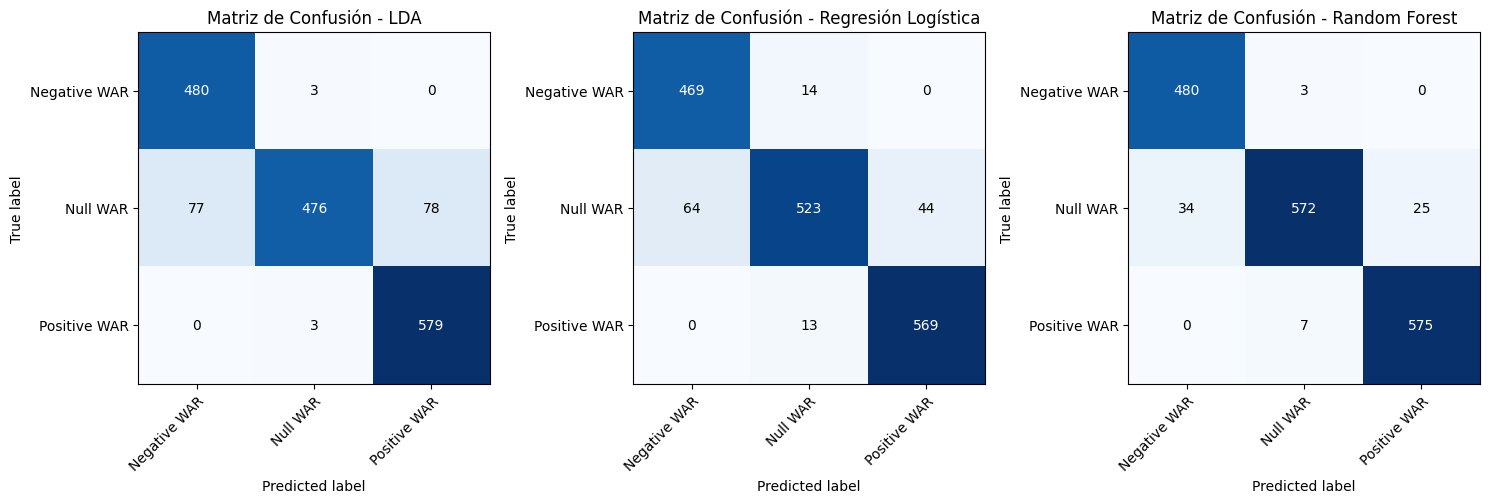
\includegraphics[width=\textwidth]{figuras/confusion_matrices.png}
    \caption{Matrices de confusión para los tres modelos evaluados en el conjunto de prueba. De izquierda a derecha: LDA, Regresión Logística y Random Forest.}
    \label{fig:confusion_matrices}
\end{figure}

El análisis de las matrices de confusión muestra que el modelo LDA tuvo dificultades particulares para clasificar la clase 2 (WAR Nulo), con 77 ejemplos incorrectamente clasificados como clase 1 y 78 como clase 3. La regresión logística mejoró ligeramente la clasificación de la clase 2, pero seguía confundiendo algunos casos con la clase 1. El Random Forest logró una clasificación mucho más precisa de todas las clases, aunque mantuvo un patrón similar de confusión entre clases adyacentes.

La comparación entre las métricas obtenidas en validación y prueba muestra una buena consistencia para los tres modelos, lo que indica que las estimaciones de error mediante validación cruzada fueron confiables. El Random Forest mostró incluso una ligera mejora en el conjunto de prueba respecto a validación (95.22\% vs 91.75\% en exactitud), posiblemente debido a que este modelo pudo aprovecharse de todo el conjunto de desarrollo para su entrenamiento final.

Es interesante notar que todas las clases muestran AUC-ROC superior a 0.97 en el caso del Random Forest, indicando una excelente capacidad de discriminación. El modelo parece captar eficientemente las relaciones entre las variables de entrada y el rendimiento de los jugadores, incluso para los casos fronterizos entre clases adyacentes.

\subsection{Discusión y Conclusiones}

La superioridad del Random Forest probablemente se debe a su capacidad para capturar relaciones no lineales entre las variables y el manejo implícito de interacciones entre características. Esto es particularmente valioso en este contexto, donde el rendimiento de un jugador de baloncesto puede depender de combinaciones complejas de sus estadísticas individuales. Además, el proceso de optimización de hiperparámetros mediante validación cruzada permitió encontrar una configuración que balancea adecuadamente la complejidad del modelo y su capacidad de generalización.

Por otro lado, tanto LDA como la regresión logística, al ser modelos lineales, tienen limitaciones inherentes para capturar patrones complejos en los datos. A pesar de esto, ambos modelos lograron un rendimiento respetable, con exactitudes superiores al 90\%, lo que sugiere que existe una estructura lineal significativa en los datos que estos modelos pudieron aprovechar.

Las métricas obtenidas en los conjuntos de validación (91.75\% para RF, 90.71\% para RL y 89.09\% para LDA) fueron consistentemente cercanas a las obtenidas en el conjunto de prueba, lo que valida la robustez de nuestro proceso de evaluación. Esta consistencia indica que las estimaciones de error mediante validación cruzada fueron confiables y representativas del rendimiento real de los modelos. En el caso de Random Forest, la ligera mejora en el conjunto de prueba podría atribuirse a la estabilidad adicional proporcionada por el entrenamiento con el conjunto completo de desarrollo.

En un entorno de producción, el modelo Random Forest sería la elección más recomendable debido a su superior rendimiento predictivo en todas las métricas. Sin embargo, si la interpretabilidad fuera un factor crítico, la regresión logística podría ser preferible, ya que sus coeficientes proporcionan información directa sobre la influencia de cada variable en la clasificación. El hecho de que nuestro modelo Random Forest alcanzara un 95.22\% de exactitud indica que es posible predecir con alta confiabilidad el impacto que un jugador tendrá en términos de victorias para su equipo basándonos únicamente en sus estadísticas individuales, lo que representa una herramienta valiosa para la gestión deportiva y la toma de decisiones estratégicas en equipos de basketball.